% Options for packages loaded elsewhere
\PassOptionsToPackage{unicode}{hyperref}
\PassOptionsToPackage{hyphens}{url}
%
\documentclass[
]{article}
\usepackage{amsmath,amssymb}
\usepackage{lmodern}
\usepackage{iftex}
\ifPDFTeX
  \usepackage[T1]{fontenc}
  \usepackage[utf8]{inputenc}
  \usepackage{textcomp} % provide euro and other symbols
\else % if luatex or xetex
  \usepackage{unicode-math}
  \defaultfontfeatures{Scale=MatchLowercase}
  \defaultfontfeatures[\rmfamily]{Ligatures=TeX,Scale=1}
\fi
% Use upquote if available, for straight quotes in verbatim environments
\IfFileExists{upquote.sty}{\usepackage{upquote}}{}
\IfFileExists{microtype.sty}{% use microtype if available
  \usepackage[]{microtype}
  \UseMicrotypeSet[protrusion]{basicmath} % disable protrusion for tt fonts
}{}
\makeatletter
\@ifundefined{KOMAClassName}{% if non-KOMA class
  \IfFileExists{parskip.sty}{%
    \usepackage{parskip}
  }{% else
    \setlength{\parindent}{0pt}
    \setlength{\parskip}{6pt plus 2pt minus 1pt}}
}{% if KOMA class
  \KOMAoptions{parskip=half}}
\makeatother
\usepackage{xcolor}
\usepackage[margin=1in]{geometry}
\usepackage{color}
\usepackage{fancyvrb}
\newcommand{\VerbBar}{|}
\newcommand{\VERB}{\Verb[commandchars=\\\{\}]}
\DefineVerbatimEnvironment{Highlighting}{Verbatim}{commandchars=\\\{\}}
% Add ',fontsize=\small' for more characters per line
\usepackage{framed}
\definecolor{shadecolor}{RGB}{248,248,248}
\newenvironment{Shaded}{\begin{snugshade}}{\end{snugshade}}
\newcommand{\AlertTok}[1]{\textcolor[rgb]{0.94,0.16,0.16}{#1}}
\newcommand{\AnnotationTok}[1]{\textcolor[rgb]{0.56,0.35,0.01}{\textbf{\textit{#1}}}}
\newcommand{\AttributeTok}[1]{\textcolor[rgb]{0.77,0.63,0.00}{#1}}
\newcommand{\BaseNTok}[1]{\textcolor[rgb]{0.00,0.00,0.81}{#1}}
\newcommand{\BuiltInTok}[1]{#1}
\newcommand{\CharTok}[1]{\textcolor[rgb]{0.31,0.60,0.02}{#1}}
\newcommand{\CommentTok}[1]{\textcolor[rgb]{0.56,0.35,0.01}{\textit{#1}}}
\newcommand{\CommentVarTok}[1]{\textcolor[rgb]{0.56,0.35,0.01}{\textbf{\textit{#1}}}}
\newcommand{\ConstantTok}[1]{\textcolor[rgb]{0.00,0.00,0.00}{#1}}
\newcommand{\ControlFlowTok}[1]{\textcolor[rgb]{0.13,0.29,0.53}{\textbf{#1}}}
\newcommand{\DataTypeTok}[1]{\textcolor[rgb]{0.13,0.29,0.53}{#1}}
\newcommand{\DecValTok}[1]{\textcolor[rgb]{0.00,0.00,0.81}{#1}}
\newcommand{\DocumentationTok}[1]{\textcolor[rgb]{0.56,0.35,0.01}{\textbf{\textit{#1}}}}
\newcommand{\ErrorTok}[1]{\textcolor[rgb]{0.64,0.00,0.00}{\textbf{#1}}}
\newcommand{\ExtensionTok}[1]{#1}
\newcommand{\FloatTok}[1]{\textcolor[rgb]{0.00,0.00,0.81}{#1}}
\newcommand{\FunctionTok}[1]{\textcolor[rgb]{0.00,0.00,0.00}{#1}}
\newcommand{\ImportTok}[1]{#1}
\newcommand{\InformationTok}[1]{\textcolor[rgb]{0.56,0.35,0.01}{\textbf{\textit{#1}}}}
\newcommand{\KeywordTok}[1]{\textcolor[rgb]{0.13,0.29,0.53}{\textbf{#1}}}
\newcommand{\NormalTok}[1]{#1}
\newcommand{\OperatorTok}[1]{\textcolor[rgb]{0.81,0.36,0.00}{\textbf{#1}}}
\newcommand{\OtherTok}[1]{\textcolor[rgb]{0.56,0.35,0.01}{#1}}
\newcommand{\PreprocessorTok}[1]{\textcolor[rgb]{0.56,0.35,0.01}{\textit{#1}}}
\newcommand{\RegionMarkerTok}[1]{#1}
\newcommand{\SpecialCharTok}[1]{\textcolor[rgb]{0.00,0.00,0.00}{#1}}
\newcommand{\SpecialStringTok}[1]{\textcolor[rgb]{0.31,0.60,0.02}{#1}}
\newcommand{\StringTok}[1]{\textcolor[rgb]{0.31,0.60,0.02}{#1}}
\newcommand{\VariableTok}[1]{\textcolor[rgb]{0.00,0.00,0.00}{#1}}
\newcommand{\VerbatimStringTok}[1]{\textcolor[rgb]{0.31,0.60,0.02}{#1}}
\newcommand{\WarningTok}[1]{\textcolor[rgb]{0.56,0.35,0.01}{\textbf{\textit{#1}}}}
\usepackage{graphicx}
\makeatletter
\def\maxwidth{\ifdim\Gin@nat@width>\linewidth\linewidth\else\Gin@nat@width\fi}
\def\maxheight{\ifdim\Gin@nat@height>\textheight\textheight\else\Gin@nat@height\fi}
\makeatother
% Scale images if necessary, so that they will not overflow the page
% margins by default, and it is still possible to overwrite the defaults
% using explicit options in \includegraphics[width, height, ...]{}
\setkeys{Gin}{width=\maxwidth,height=\maxheight,keepaspectratio}
% Set default figure placement to htbp
\makeatletter
\def\fps@figure{htbp}
\makeatother
\setlength{\emergencystretch}{3em} % prevent overfull lines
\providecommand{\tightlist}{%
  \setlength{\itemsep}{0pt}\setlength{\parskip}{0pt}}
\setcounter{secnumdepth}{-\maxdimen} % remove section numbering
\usepackage{booktabs}
\usepackage{longtable}
\usepackage{array}
\usepackage{multirow}
\usepackage{wrapfig}
\usepackage{float}
\usepackage{colortbl}
\usepackage{pdflscape}
\usepackage{tabu}
\usepackage{threeparttable}
\usepackage{threeparttablex}
\usepackage[normalem]{ulem}
\usepackage{makecell}
\usepackage{xcolor}
\ifLuaTeX
  \usepackage{selnolig}  % disable illegal ligatures
\fi
\IfFileExists{bookmark.sty}{\usepackage{bookmark}}{\usepackage{hyperref}}
\IfFileExists{xurl.sty}{\usepackage{xurl}}{} % add URL line breaks if available
\urlstyle{same} % disable monospaced font for URLs
\hypersetup{
  pdftitle={COS-D419 Factor Analysis and Structural Equation Models 2023, Assignment 2},
  pdfauthor={Rong Guang},
  hidelinks,
  pdfcreator={LaTeX via pandoc}}

\title{COS-D419 Factor Analysis and Structural Equation Models 2023,
Assignment 2}
\author{Rong Guang}
\date{2023-01-30}

\begin{document}
\maketitle

\hypertarget{exercise-2.1}{%
\section{1 Exercise 2.1}\label{exercise-2.1}}

Specify and test the hypothesis given on the page 1 of the lecture
material.

Draw conclusions based on the \(\chi^2\) statistic and the CFI, TLI,
RMSEA, and SRMR indices.

What can you say about the parameter estimates?

Visualize the model.

\hypertarget{read-in-the-data-set}{%
\subsection{1.1 Read in the data set}\label{read-in-the-data-set}}

Start by downloading the data file from Moodle to Project folder.

\begin{Shaded}
\begin{Highlighting}[]
\FunctionTok{library}\NormalTok{(tidyverse)}\CommentTok{\#data wrangling }
\FunctionTok{library}\NormalTok{(readr)}\CommentTok{\# read data into r}
\NormalTok{orig\_data }\OtherTok{\textless{}{-}} \FunctionTok{read\_csv}\NormalTok{(}\StringTok{"ASC7INDM.CSV"}\NormalTok{, }\AttributeTok{show\_col\_types =} \ConstantTok{FALSE}\NormalTok{) }
\end{Highlighting}
\end{Shaded}

\hypertarget{write-functions}{%
\subsection{1.2 Write functions}\label{write-functions}}

\begin{Shaded}
\begin{Highlighting}[]
\NormalTok{unique.levels }\OtherTok{\textless{}{-}}  \ControlFlowTok{function}\NormalTok{(sc)\{}
\NormalTok{  values }\OtherTok{\textless{}{-}} \FunctionTok{lapply}\NormalTok{(sc, }\ControlFlowTok{function}\NormalTok{(x)}\FunctionTok{sort}\NormalTok{(}\FunctionTok{unique}\NormalTok{(x))) }
\ControlFlowTok{for}\NormalTok{(x }\ControlFlowTok{in} \DecValTok{1}\SpecialCharTok{:}\FunctionTok{ncol}\NormalTok{(sc))\{}
\NormalTok{  a }\OtherTok{\textless{}{-}} \FunctionTok{paste}\NormalTok{(}\FunctionTok{c}\NormalTok{(}\StringTok{"Variable "}\NormalTok{, }
               \FunctionTok{names}\NormalTok{(values)[x], }
               \StringTok{" has values of "}\NormalTok{, }
               \FunctionTok{paste}\NormalTok{(values[[x]], }
                     \AttributeTok{collapse =} \StringTok{","}\NormalTok{)), }
             \AttributeTok{collapse =} \StringTok{""}\NormalTok{)}
  \FunctionTok{print}\NormalTok{(a)}
\NormalTok{  \}}
\NormalTok{\}}
\end{Highlighting}
\end{Shaded}

\hypertarget{subset-the-data-set}{%
\subsection{1.3 Subset the data set}\label{subset-the-data-set}}

Subset the variables for analysis and name it as sc (Self-concept).

\begin{Shaded}
\begin{Highlighting}[]
\CommentTok{\# Select the variables for use}
\NormalTok{sc }\OtherTok{\textless{}{-}}\NormalTok{ orig\_data }\SpecialCharTok{\%\textgreater{}\%}\NormalTok{ dplyr}\SpecialCharTok{::}\FunctionTok{select}\NormalTok{(}\FunctionTok{starts\_with}\NormalTok{(}\StringTok{"SDQ2N"}\NormalTok{)) }\CommentTok{\# namming logic: sc = self{-}concept}
\end{Highlighting}
\end{Shaded}

\hypertarget{inspect-the-data}{%
\subsection{1.4 Inspect the data}\label{inspect-the-data}}

Have a quick overview of the data.

\begin{Shaded}
\begin{Highlighting}[]
\FunctionTok{glimpse}\NormalTok{(sc)}
\end{Highlighting}
\end{Shaded}

\begin{verbatim}
## Rows: 265
## Columns: 16
## $ SDQ2N01 <dbl> 6, 6, 4, 5, 6, 5, 1, 2, 5, 4, 2, 5, 6, 4, 4, 6, 6, 6, 5, 6, 6,~
## $ SDQ2N13 <dbl> 5, 6, 6, 5, 5, 5, 6, 1, 5, 6, 6, 5, 6, 3, 5, 6, 6, 6, 4, 5, 5,~
## $ SDQ2N25 <dbl> 4, 6, 6, 5, 5, 5, 1, 6, 6, 3, 6, 6, 6, 5, 5, 6, 6, 6, 6, 5, 4,~
## $ SDQ2N37 <dbl> 6, 6, 2, 6, 4, 3, 6, 4, 6, 6, 6, 5, 5, 5, 4, 5, 6, 4, 4, 6, 6,~
## $ SDQ2N04 <dbl> 3, 6, 6, 5, 3, 3, 4, 4, 6, 6, 5, 6, 5, 4, 4, 4, 4, 6, 5, 5, 3,~
## $ SDQ2N16 <dbl> 4, 6, 4, 6, 4, 2, 6, 4, 6, 5, 6, 6, 5, 5, 5, 5, 6, 5, 4, 6, 6,~
## $ SDQ2N28 <dbl> 4, 6, 6, 5, 4, 4, 6, 4, 6, 6, 6, 6, 5, 5, 5, 5, 6, 4, 2, 4, 4,~
## $ SDQ2N40 <dbl> 6, 6, 3, 6, 4, 4, 6, 6, 6, 6, 6, 6, 6, 5, 4, 4, 6, 6, 5, 5, 5,~
## $ SDQ2N10 <dbl> 2, 5, 6, 5, 4, 4, 1, 6, 5, 4, 2, 6, 5, 5, 5, 3, 4, 6, 5, 4, 6,~
## $ SDQ2N22 <dbl> 6, 6, 5, 6, 6, 4, 6, 6, 6, 6, 6, 6, 6, 5, 6, 6, 6, 6, 6, 3, 6,~
## $ SDQ2N34 <dbl> 1, 6, 4, 3, 5, 5, 1, 1, 5, 4, 5, 6, 5, 2, 5, 2, 3, 2, 1, 3, 3,~
## $ SDQ2N46 <dbl> 5, 6, 5, 5, 6, 6, 6, 5, 6, 6, 6, 6, 6, 6, 2, 5, 6, 6, 6, 6, 6,~
## $ SDQ2N07 <dbl> 6, 6, 6, 6, 3, 4, 5, 3, 6, 5, 6, 6, 6, 6, 4, 4, 6, 6, 6, 6, 3,~
## $ SDQ2N19 <dbl> 6, 6, 6, 6, 4, 5, 6, 4, 6, 6, 5, 6, 6, 6, 5, 5, 6, 6, 5, 5, 5,~
## $ SDQ2N31 <dbl> 6, 6, 3, 6, 4, 4, 6, 4, 6, 6, 6, 6, 6, 6, 5, 5, 6, 6, 5, 5, 5,~
## $ SDQ2N43 <dbl> 6, 6, 1, 5, 5, 4, 5, 6, 6, 6, 6, 6, 6, 6, 5, 6, 6, 6, 5, 6, 5,~
\end{verbatim}

The data set includes 16 variables from 265 observations. All the
variables are numeric. Next, I examined the unique values of each
variables.

\begin{Shaded}
\begin{Highlighting}[]
\FunctionTok{unique.levels}\NormalTok{(sc)}
\end{Highlighting}
\end{Shaded}

\begin{verbatim}
## [1] "Variable SDQ2N01 has values of 1,2,3,4,5,6"
## [1] "Variable SDQ2N13 has values of 1,2,3,4,5,6"
## [1] "Variable SDQ2N25 has values of 1,2,3,4,5,6"
## [1] "Variable SDQ2N37 has values of 1,2,3,4,5,6"
## [1] "Variable SDQ2N04 has values of 1,2,3,4,5,6"
## [1] "Variable SDQ2N16 has values of 1,2,3,4,5,6"
## [1] "Variable SDQ2N28 has values of 1,2,3,4,5,6"
## [1] "Variable SDQ2N40 has values of 1,2,3,4,5,6"
## [1] "Variable SDQ2N10 has values of 1,2,3,4,5,6"
## [1] "Variable SDQ2N22 has values of 1,2,3,4,5,6"
## [1] "Variable SDQ2N34 has values of 1,2,3,4,5,6"
## [1] "Variable SDQ2N46 has values of 1,2,3,4,5,6"
## [1] "Variable SDQ2N07 has values of 1,2,3,4,5,6"
## [1] "Variable SDQ2N19 has values of 1,2,3,4,5,6"
## [1] "Variable SDQ2N31 has values of 1,2,3,4,5,6"
## [1] "Variable SDQ2N43 has values of 1,2,3,4,5,6"
\end{verbatim}

For each variable, the values distribute from 1 to 6.

\hypertarget{explore-the-data}{%
\section{2 Explore the data}\label{explore-the-data}}

\hypertarget{descriptive-statistics}{%
\subsection{2.1 Descriptive statistics}\label{descriptive-statistics}}

\begin{Shaded}
\begin{Highlighting}[]
\FunctionTok{library}\NormalTok{(kableExtra)}\CommentTok{\#improved table visuals}
\FunctionTok{library}\NormalTok{(psych)}\CommentTok{\#for function "describe"}
\NormalTok{sc.ds }\OtherTok{\textless{}{-}}\NormalTok{ sc }\SpecialCharTok{\%\textgreater{}\%}  \CommentTok{\#sc.ds = self{-}concept descriptive statistics}
  \FunctionTok{describe}\NormalTok{(}\AttributeTok{IQR =}\NormalTok{ T) }\SpecialCharTok{\%\textgreater{}\%}
  \FunctionTok{as.data.frame}\NormalTok{() }\SpecialCharTok{\%\textgreater{}\%} 
\NormalTok{  dplyr}\SpecialCharTok{::}\FunctionTok{select}\NormalTok{(mean, median, sd, range, se, IQR)}
\CommentTok{\#print the descriptive statistics table}
\NormalTok{sc.ds }\SpecialCharTok{\%\textgreater{}\%} 
  \FunctionTok{kable}\NormalTok{(}\AttributeTok{booktabs=}\NormalTok{T,}
        \AttributeTok{longtable=}\NormalTok{T,}
        \AttributeTok{digits =} \DecValTok{2}\NormalTok{,}
        \AttributeTok{caption =} \StringTok{"Descriptive dtatistics of selected variables"}\NormalTok{,}
        \AttributeTok{linesep =} \StringTok{""}\NormalTok{) }\SpecialCharTok{\%\textgreater{}\%} 
  \FunctionTok{add\_header\_above}\NormalTok{(}\FunctionTok{c}\NormalTok{(}\StringTok{""}\NormalTok{, }\StringTok{"centralized tendency"} \OtherTok{=} \DecValTok{2}\NormalTok{, }\StringTok{"dispersion tendency"} \OtherTok{=} \DecValTok{4}\NormalTok{)) }\SpecialCharTok{\%\textgreater{}\%} 
  \FunctionTok{kable\_styling}\NormalTok{(}\AttributeTok{latex\_options =} \FunctionTok{c}\NormalTok{(}\StringTok{"striped"}\NormalTok{,}\StringTok{"repeat\_header"}\NormalTok{)) }\SpecialCharTok{\%\textgreater{}\%} 
  \FunctionTok{column\_spec}\NormalTok{(}\DecValTok{1}\NormalTok{, }\AttributeTok{width =} \StringTok{"3cm"}\NormalTok{, }\AttributeTok{bold =}\NormalTok{ T, }\AttributeTok{color =} \StringTok{"red"}\NormalTok{)}
\end{Highlighting}
\end{Shaded}

\begin{longtable}[t]{>{\raggedright\arraybackslash}p{3cm}rrrrrr}
\caption{\label{tab:unnamed-chunk-6}Descriptive dtatistics of selected variables}\\
\toprule
\multicolumn{1}{c}{} & \multicolumn{2}{c}{centralized tendency} & \multicolumn{4}{c}{dispersion tendency} \\
\cmidrule(l{3pt}r{3pt}){2-3} \cmidrule(l{3pt}r{3pt}){4-7}
  & mean & median & sd & range & se & IQR\\
\midrule
\endfirsthead
\caption[]{Descriptive dtatistics of selected variables \textit{(continued)}}\\
\toprule
\multicolumn{1}{c}{} & \multicolumn{2}{c}{centralized tendency} & \multicolumn{4}{c}{dispersion tendency} \\
\cmidrule(l{3pt}r{3pt}){2-3} \cmidrule(l{3pt}r{3pt}){4-7}
  & mean & median & sd & range & se & IQR\\
\midrule
\endhead

\endfoot
\bottomrule
\endlastfoot
\textcolor{red}{\textbf{\cellcolor{gray!6}{SDQ2N01}}} & \cellcolor{gray!6}{4.41} & \cellcolor{gray!6}{5} & \cellcolor{gray!6}{1.35} & \cellcolor{gray!6}{5} & \cellcolor{gray!6}{0.08} & \cellcolor{gray!6}{1}\\
\textcolor{red}{\textbf{SDQ2N13}} & 5.00 & 6 & 1.36 & 5 & 0.08 & 2\\
\textcolor{red}{\textbf{\cellcolor{gray!6}{SDQ2N25}}} & \cellcolor{gray!6}{5.10} & \cellcolor{gray!6}{6} & \cellcolor{gray!6}{1.23} & \cellcolor{gray!6}{5} & \cellcolor{gray!6}{0.08} & \cellcolor{gray!6}{1}\\
\textcolor{red}{\textbf{SDQ2N37}} & 4.83 & 5 & 1.14 & 5 & 0.07 & 2\\
\textcolor{red}{\textbf{\cellcolor{gray!6}{SDQ2N04}}} & \cellcolor{gray!6}{4.52} & \cellcolor{gray!6}{5} & \cellcolor{gray!6}{1.40} & \cellcolor{gray!6}{5} & \cellcolor{gray!6}{0.09} & \cellcolor{gray!6}{2}\\
\textcolor{red}{\textbf{SDQ2N16}} & 4.65 & 5 & 1.24 & 5 & 0.08 & 2\\
\textcolor{red}{\textbf{\cellcolor{gray!6}{SDQ2N28}}} & \cellcolor{gray!6}{4.69} & \cellcolor{gray!6}{5} & \cellcolor{gray!6}{1.33} & \cellcolor{gray!6}{5} & \cellcolor{gray!6}{0.08} & \cellcolor{gray!6}{2}\\
\textcolor{red}{\textbf{SDQ2N40}} & 4.98 & 5 & 1.36 & 5 & 0.08 & 1\\
\textcolor{red}{\textbf{\cellcolor{gray!6}{SDQ2N10}}} & \cellcolor{gray!6}{4.62} & \cellcolor{gray!6}{5} & \cellcolor{gray!6}{1.15} & \cellcolor{gray!6}{5} & \cellcolor{gray!6}{0.07} & \cellcolor{gray!6}{1}\\
\textcolor{red}{\textbf{SDQ2N22}} & 5.38 & 6 & 1.09 & 5 & 0.07 & 1\\
\textcolor{red}{\textbf{\cellcolor{gray!6}{SDQ2N34}}} & \cellcolor{gray!6}{3.89} & \cellcolor{gray!6}{4} & \cellcolor{gray!6}{1.70} & \cellcolor{gray!6}{5} & \cellcolor{gray!6}{0.10} & \cellcolor{gray!6}{3}\\
\textcolor{red}{\textbf{SDQ2N46}} & 5.27 & 6 & 1.30 & 5 & 0.08 & 1\\
\textcolor{red}{\textbf{\cellcolor{gray!6}{SDQ2N07}}} & \cellcolor{gray!6}{4.32} & \cellcolor{gray!6}{5} & \cellcolor{gray!6}{1.78} & \cellcolor{gray!6}{5} & \cellcolor{gray!6}{0.11} & \cellcolor{gray!6}{3}\\
\textcolor{red}{\textbf{SDQ2N19}} & 4.54 & 5 & 1.69 & 5 & 0.10 & 2\\
\textcolor{red}{\textbf{\cellcolor{gray!6}{SDQ2N31}}} & \cellcolor{gray!6}{4.74} & \cellcolor{gray!6}{5} & \cellcolor{gray!6}{1.57} & \cellcolor{gray!6}{5} & \cellcolor{gray!6}{0.10} & \cellcolor{gray!6}{2}\\
\textcolor{red}{\textbf{SDQ2N43}} & 4.98 & 5 & 1.40 & 5 & 0.09 & 1\\*
\end{longtable}

\begin{Shaded}
\begin{Highlighting}[]
\CommentTok{\#sc.ds \%\textgreater{}\%}
\CommentTok{\#  tab\_df(digits = 2, }
\CommentTok{\#        alternate.rows = T,}
\CommentTok{\#        title = "Table 1. Descriptive dtatistics of selected variables",}
\CommentTok{\#        CSS = list(css.centralign=\textquotesingle{}text{-}align: right;\textquotesingle{}))}
\end{Highlighting}
\end{Shaded}

\hypertarget{visualization}{%
\subsection{2.2 Visualization}\label{visualization}}

\hypertarget{histogram}{%
\subsubsection{2.2.1 Histogram}\label{histogram}}

\begin{Shaded}
\begin{Highlighting}[]
\NormalTok{sc }\SpecialCharTok{\%\textgreater{}\%} 
  \FunctionTok{pivot\_longer}\NormalTok{(}\FunctionTok{everything}\NormalTok{()) }\SpecialCharTok{\%\textgreater{}\%}  \CommentTok{\#longer format}
  \FunctionTok{ggplot}\NormalTok{(}\FunctionTok{aes}\NormalTok{(}\AttributeTok{x =}\NormalTok{ value)) }\SpecialCharTok{+} \CommentTok{\#x axis used variable "value" (a default of pivot)}
  \FunctionTok{geom\_histogram}\NormalTok{(}\AttributeTok{binwidth =} \DecValTok{1}\NormalTok{, }\FunctionTok{aes}\NormalTok{(}\AttributeTok{y =}\NormalTok{ ..density..), }\CommentTok{\#match ys of density and histogram plots}
                 \AttributeTok{color =} \StringTok{"black"}\NormalTok{,  }\AttributeTok{fill =} \StringTok{"\#9999CC"}\NormalTok{)}\SpecialCharTok{+}  \CommentTok{\# adjust aesthetics for hist}
  \FunctionTok{geom\_density}\NormalTok{(}\AttributeTok{fill =} \StringTok{"pink"}\NormalTok{, }\AttributeTok{alpha =} \FloatTok{0.25}\NormalTok{)}\SpecialCharTok{+} \CommentTok{\#adjust aesthetics for density plot}
  \FunctionTok{facet\_wrap}\NormalTok{(}\SpecialCharTok{\textasciitilde{}}\NormalTok{name, }\AttributeTok{scales =} \StringTok{"free"}\NormalTok{) }\SpecialCharTok{+} \CommentTok{\#wrap by name variable}
  \FunctionTok{theme}\NormalTok{(}\AttributeTok{panel.grid.major =} \FunctionTok{element\_blank}\NormalTok{(), }\CommentTok{\#get rid of the  grids}
        \AttributeTok{panel.grid.minor =} \FunctionTok{element\_blank}\NormalTok{(),}
        \AttributeTok{panel.background =} \FunctionTok{element\_rect}\NormalTok{(}\AttributeTok{fill =} \StringTok{"white"}\NormalTok{,}\CommentTok{\#adjust the background}
                                        \AttributeTok{color =} \StringTok{"black"}\NormalTok{),}
        \AttributeTok{strip.background =} \FunctionTok{element\_rect}\NormalTok{(}\AttributeTok{color =} \StringTok{"black"}\NormalTok{,}\CommentTok{\#adjust the strips aes}
                                        \AttributeTok{fill =} \StringTok{"steelblue"}\NormalTok{),}
        \AttributeTok{strip.text =} \FunctionTok{element\_text}\NormalTok{(}\AttributeTok{size =}\DecValTok{8}\NormalTok{, }\AttributeTok{color =} \StringTok{"white"}\NormalTok{), }\CommentTok{\#adjust strip text}
        \AttributeTok{axis.title.x =} \FunctionTok{element\_text}\NormalTok{(}\AttributeTok{size =} \DecValTok{3}\NormalTok{), }\CommentTok{\#adjust the x text}
        \AttributeTok{axis.title.y =} \FunctionTok{element\_text}\NormalTok{(}\AttributeTok{size =} \DecValTok{3}\NormalTok{), }\CommentTok{\# adjust the y text}
        \AttributeTok{plot.title =} \FunctionTok{element\_text}\NormalTok{(}\AttributeTok{size =} \DecValTok{12}\NormalTok{, }\AttributeTok{face =} \StringTok{"bold"}\NormalTok{))}\SpecialCharTok{+} \CommentTok{\#adjust the title}
  \FunctionTok{labs}\NormalTok{(}\AttributeTok{title =} \StringTok{"Figure 1 Distribution of selected items"}\NormalTok{) }\CommentTok{\#title it}
\end{Highlighting}
\end{Shaded}

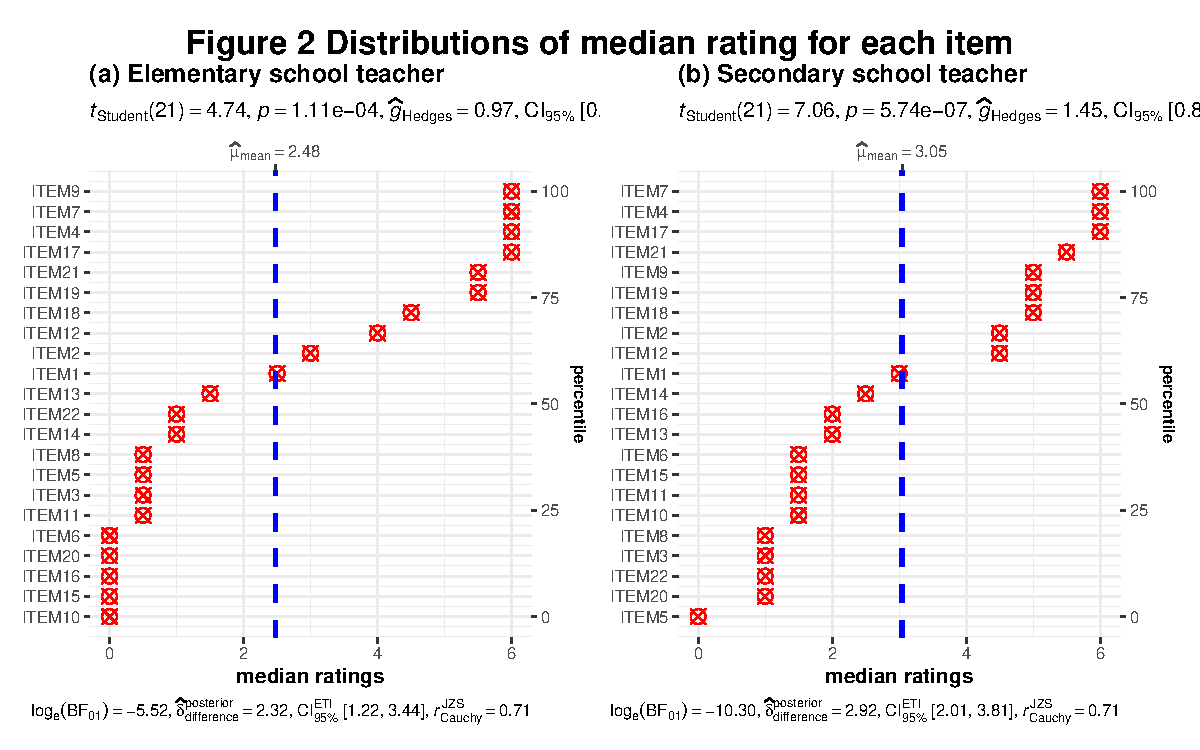
\includegraphics{Assignment2_RongGuang_files/figure-latex/unnamed-chunk-7-1.pdf}

\hypertarget{correlation-plot}{%
\subsubsection{2.2.2 Correlation plot}\label{correlation-plot}}

\begin{Shaded}
\begin{Highlighting}[]
\FunctionTok{library}\NormalTok{(GGally)}
\FunctionTok{ggcorr}\NormalTok{(sc, }
       \AttributeTok{geom =} \StringTok{"blank"}\NormalTok{, }
       \AttributeTok{label =} \ConstantTok{TRUE}\NormalTok{, }
       \AttributeTok{hjust =} \FloatTok{0.85}\NormalTok{, }
       \AttributeTok{color =} \StringTok{"red"}\NormalTok{, }
       \AttributeTok{face =} \StringTok{"bold"}\NormalTok{, }
       \AttributeTok{method =} \FunctionTok{c}\NormalTok{(}\StringTok{"pairwise"}\NormalTok{,}\StringTok{"spearman"}\NormalTok{),}
       \AttributeTok{digits =} \DecValTok{2}\NormalTok{,}
       \AttributeTok{label\_size =} \FloatTok{2.5}\NormalTok{,}
       \AttributeTok{label\_round =} \DecValTok{2}\NormalTok{) }\SpecialCharTok{+}
  \FunctionTok{geom\_point}\NormalTok{(}\AttributeTok{size =} \DecValTok{9}\NormalTok{, }
             \FunctionTok{aes}\NormalTok{(}\AttributeTok{color =} \StringTok{"red"}\NormalTok{, }
                 \AttributeTok{alpha =} \FunctionTok{abs}\NormalTok{(coefficient) }\SpecialCharTok{\textgreater{}} \FloatTok{0.3}\NormalTok{)) }\SpecialCharTok{+}
  \FunctionTok{scale\_alpha\_manual}\NormalTok{(}\AttributeTok{values =} \FunctionTok{c}\NormalTok{(}\StringTok{"TRUE"} \OtherTok{=} \FloatTok{0.3}\NormalTok{, }\StringTok{"FALSE"} \OtherTok{=} \DecValTok{0}\NormalTok{)) }\SpecialCharTok{+}
    \FunctionTok{geom\_point}\NormalTok{(}\AttributeTok{size =} \DecValTok{10}\NormalTok{, }
               \FunctionTok{aes}\NormalTok{(}\AttributeTok{color =} \StringTok{"green"}\NormalTok{, }\AttributeTok{alpha =} \FunctionTok{abs}\NormalTok{(coefficient) }\SpecialCharTok{\textgreater{}} \FloatTok{0.6}\NormalTok{)) }\SpecialCharTok{+}
  \FunctionTok{scale\_alpha\_manual}\NormalTok{(}\AttributeTok{values =} \FunctionTok{c}\NormalTok{(}\StringTok{"TRUE"} \OtherTok{=} \FloatTok{0.5}\NormalTok{, }\StringTok{"FALSE"} \OtherTok{=} \DecValTok{0}\NormalTok{)) }\SpecialCharTok{+}
  \FunctionTok{guides}\NormalTok{(}\AttributeTok{color =} \ConstantTok{FALSE}\NormalTok{, }
         \AttributeTok{alpha =} \ConstantTok{FALSE}\NormalTok{) }\SpecialCharTok{+}
  \FunctionTok{labs}\NormalTok{(}\AttributeTok{title =} \StringTok{"Figure 2. Spearman correlation matrix of the selected items"}\NormalTok{,}
       \AttributeTok{caption =} 
         \StringTok{"Red circles indicates correlation coefficient ≥ 0.5; gree circle indicates ≥ 0.3"}\NormalTok{)}
\end{Highlighting}
\end{Shaded}

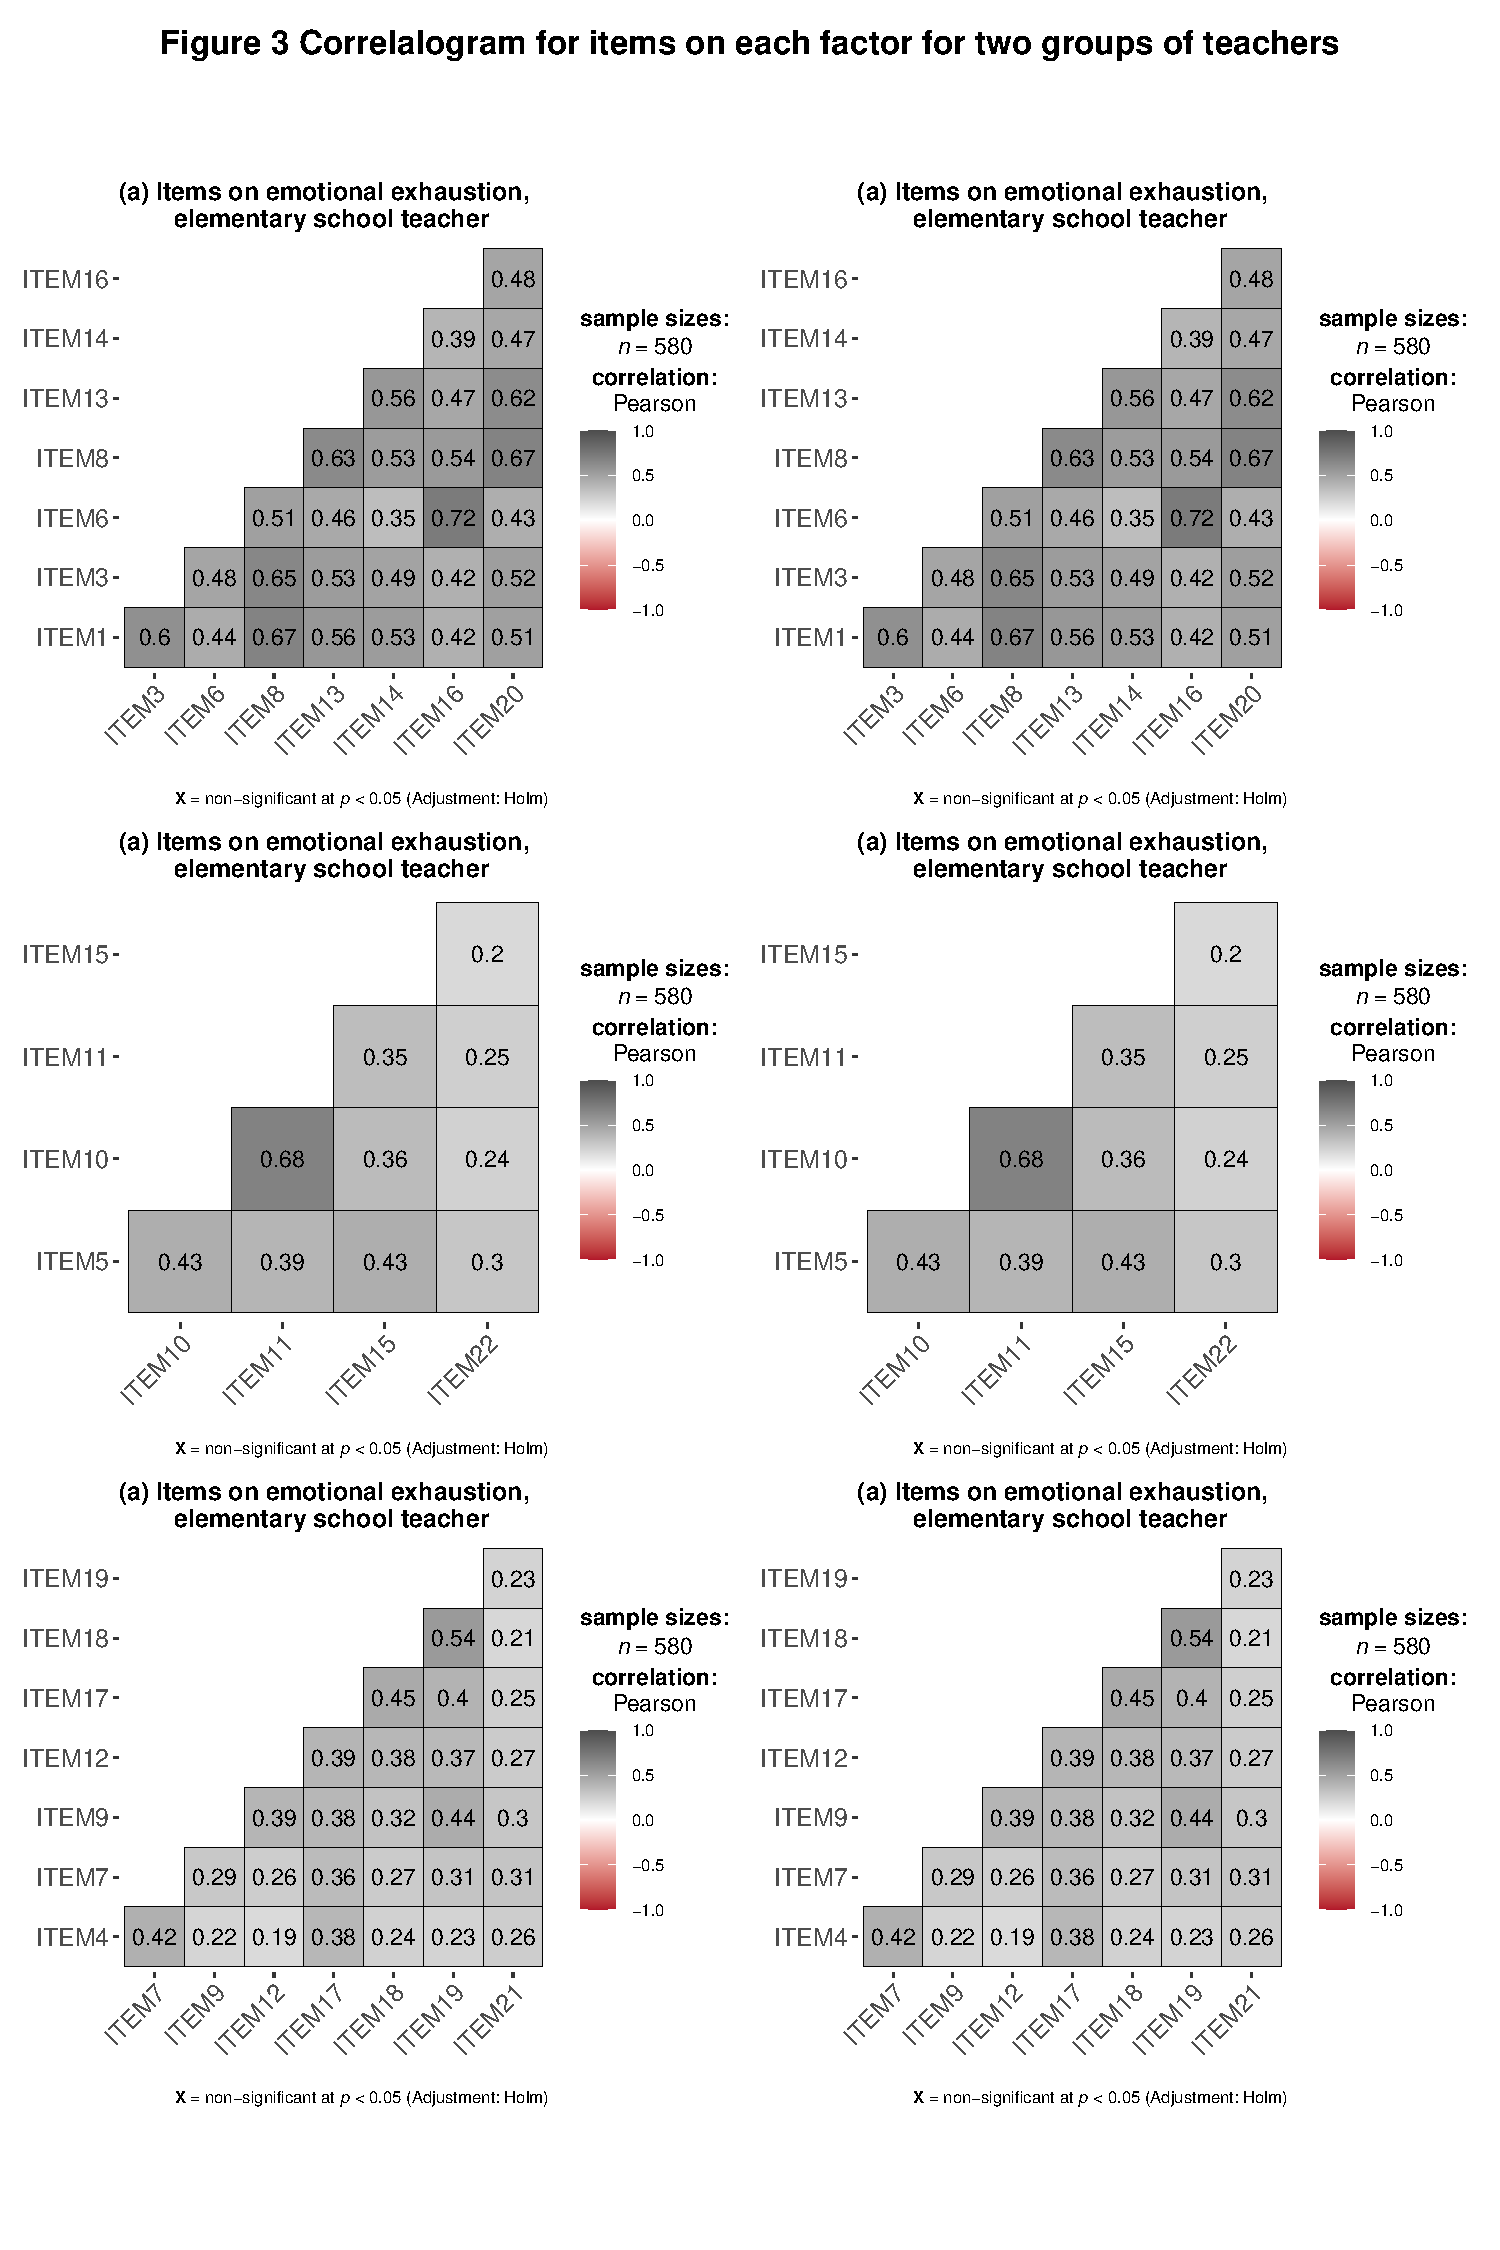
\includegraphics{Assignment2_RongGuang_files/figure-latex/unnamed-chunk-8-1.pdf}
It is found that each variable correlated with at least one of the other
variable with a spearman correlation coefficient ≥0.3, except for item
SDQ2N46 and SDQ2N34.

\end{document}
